%\documentclass[12pt,a4paper]{article}
\documentclass[12pt,a4paper]{mitthesis}
\usepackage[utf8]{inputenc}
\usepackage[spanish]{babel}

\usepackage{cite}

\usepackage{amsmath}
\usepackage{amsfonts}
\usepackage{amssymb}
\usepackage{graphicx}

\usepackage{cmap}
\pagestyle{plain}

\usepackage{pdfpages}

\usepackage{listings}
\usepackage{color}

\usepackage{tcolorbox}

%%%%%%%%%%%%%%%%%%%%%%%%%%%%%%%%%%%%%%%%%%%%%%%%%%%%%%%%%%%%%%%%%%%%%%%%%%%%%%%%%%%%%%%%%%%%%%%%%%%
%%%%%%%%%%%%%%%%%%%%%%%%%%%%%%%%%%%%%%%%%%%%%%%%%%%%%%%%%%%%%%%%%%%%%%%%%%%%%%%%%%%%%%%%%%%%%%%%%%%

\begin{document}
\pagestyle{plain}

\newtheorem{defn}{Definici\'on}

\newcommand{\R}{\mathbb{R}}
\newcommand{\Var}[1]{\mathrm{Var}\left( #1 \right)}
\newcommand{\Cov}[1]{\mathrm{Cov}\left( #1 \right)}

%%%%%%%%%%%%%%%%%%%%%%%%%%%%%%%%%%%%%%%%%%%%%%%%%%%%%%%%%%%%%%%%%%%%%%%%%%%%%%%%%%%%%%%%%%%%%%%%%%%

\tableofcontents
\newpage
%\listoffigures
%\newpage
%\listoftables

%%%%%%%%%%%%%%%%%%%%%%%%%%%%%%%%%%%%%%%%%%%%%%%%%%%%%%%%%%%%%%%%%%%%%%%%%%%%%%%%%%%%%%%%%%%%%%%%%%%

\chapter{Introducci\'on}

A grosso modo:

El objetivo de este trabajo es explorar la hip\'otesis de estacionariedad en registros
polisomnogr\'aficos (EEG durante el sue\~no) en adultos mayores con Deterioro Cognitivo y de
un grupo control.

Se describen diferencias entre [lo que arrojan los an\'alisis para] registros de ambos grupos, 
que sugieren su posible utilizaci\'on 
como marcadores de uso cl\'inico.

El estudio y diagnóstico de una gran cantidad de enfermedades depende de nuestra habilidad para
registrar y analizar se\~nales electrofisiol\'ogicas. 

Se suele asumir que estas se\~nales son complejas: no lineales, no estacionarias y sin equilibrio 
por naturaleza. Pero usualmente no se comprueban formalmente estas propiedades.

Correlaci\'on inter-hemisf\'erica durante el sueño MOR del Adulto Mayor con Deterioro Cognitivo.

\begin{figure}[h]
\centering
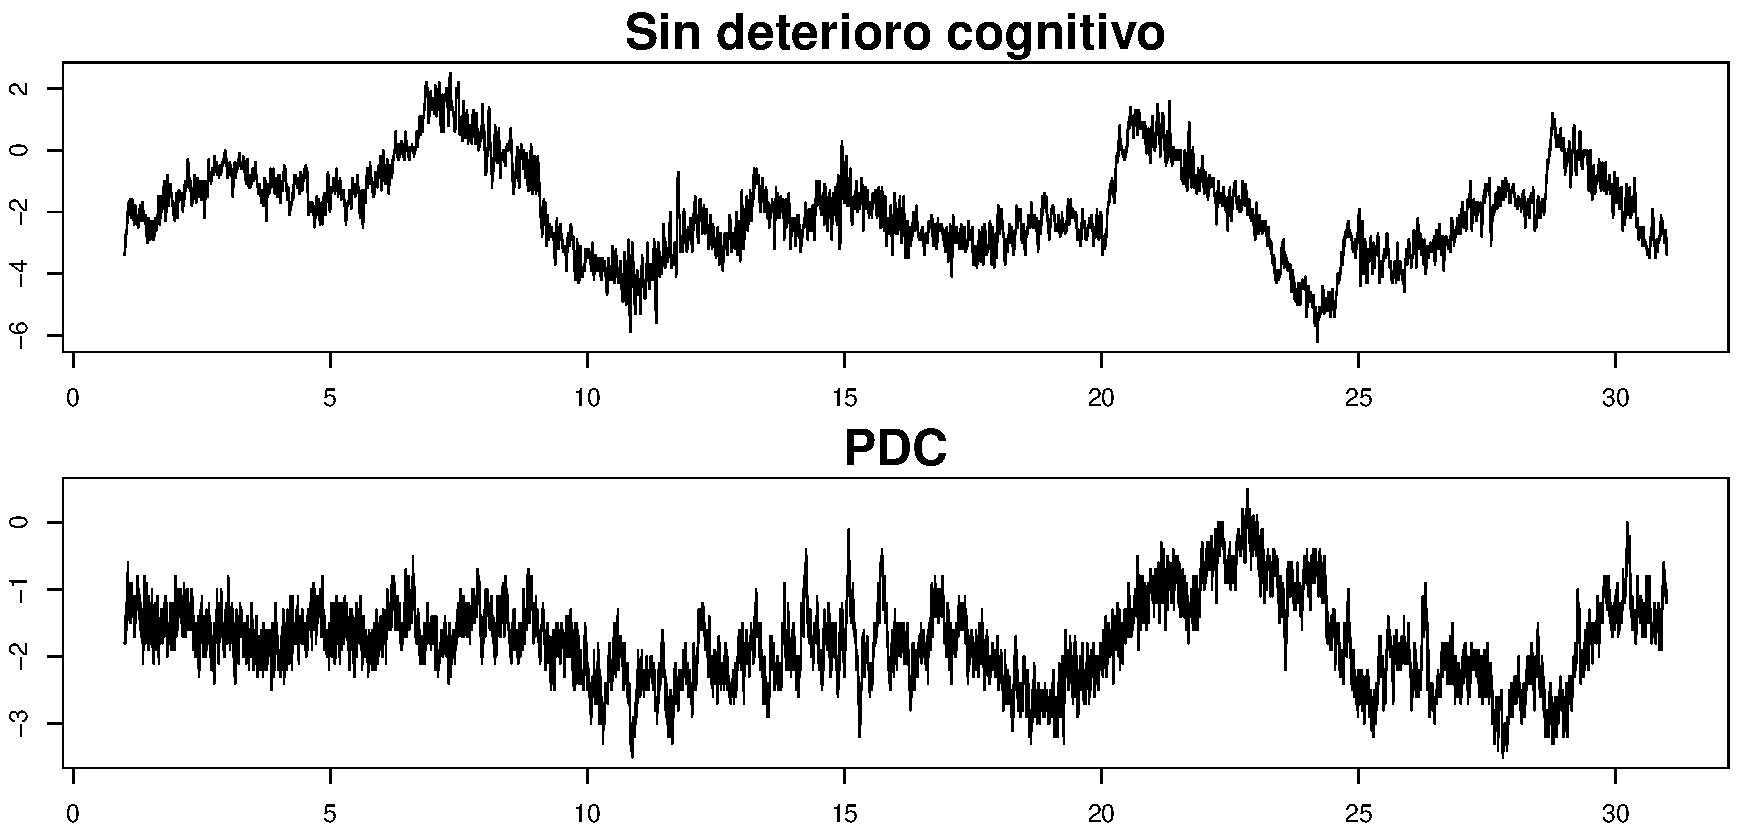
\includegraphics[width=.8\linewidth]{graficaintro.pdf}
\end{figure}

Adaptado de V\'azquez-Tagle y colaboradores (2016)

%Visualmente, el sue\~no MOR se caracteriza por movimientos oculares r\'apidos, aton\'ia muscular y 
%una actividad electroencefalogr\'afica desincronizada \cite{RosalesLagarde09}.

%%%%%%%%%%%%%%%%%%%%%%%%%%%%%%%%%%%%%%%%%%%%%%%%%%%%%%%%%%%%%%%%%%%%%%%%%%%%%%%%%%%%%%%%%%%%%%%%%%%

\chapter{''Parte fisiol\'ogica''}

Esta parte tiene partes copiadas del protocolo de G\'enesis: es temporal. Tiene mucho sentido
que, como la tesis tiene enfoque matem\'atico, deba citar el trabajo de personas enfocadas al
\'area de fisiolog\'ia. Dentro de poco escribir\'e mi propia revisi\'on, aunque sea de la misma
bibliograf\'ia.

\section{Morfolog\'a neuronal y cambios en la anatomía cerebral con la vejez (fisiolog\'ia)}

El envejecimiento considerado normal viene determinado por una serie de procesos moleculares, 
celulares, fisiol\'ogicos y psicol\'ogicos que conducen directamente al deterioro de funciones 
cognitivas, específicamente en la atenci\'on y memoria \cite{Navarrete03,Park09}.

En un principio se consideraba que el envejecimiento cerebral ocurr\'ia fundamentalmente por una 
muerte neuronal programada \cite{Coleman87}, sin embargo, estudios realizados con tejido cerebral 
post mortem de adultos mayores que en vida fueron sanos, mostraron que dicha muerte neuronal no 
alcanza un 10\% en su totalidad \cite{Esiri07}. En este sentido, los cambios morfol\'gicos que 
sufren las neuronas durante el envejecimiento son abundantes, observ\'andose una importante 
disminuci\'on de la arborizaci\'n dendr\'itica as\'i como en la densidad y volumen \cite{Hita14}. 
La disminución en la arborización dendr\'itica y de las espinas dendr\'iticas de las neuronas 
piramidales de la corteza prefrontal, temporal superior, pre central y occipital \cite{Hita14}. 
Dichas alteraciones morfol\'ogicas conducen durante el envejecimiento a una disminuci\'on de 
la densidad sin\'aptica y a una desmielinizaci\'on ax\'onica en neuronas de la 
neocorteza \cite{Terry}.

Con el paso del tiempo, la organizaci\'on an\'atomo-funcional del cerebro sufre modificaciones 
que traen como consecuencia la afectaci\'on de diferentes capacidades cognitivas, sin embargo, 
la vulnerabilidad de los circuitos neuronales ante los procesos que ocurren durante el 
envejecimiento no suceden de forma homogénea en todo el cerebro \cite{Hita14}.

Por otro lado, la relevancia del estudio de los cambios anat\'omicos asociados al envejecimiento 
fisiol\'ogico ha ido aumentando al permitir evaluar como dichos cambios se correlacionan con 
el deterioro funcional y cognitivo que caracteriza a las personas mayores, facilita la 
identificaci\'on de estadios tempranos de diferentes patolog\'ias neurodegenerativas estableciendo 
diferencias entre estas y los cambios asociados al envejecimiento fisiol\'ogico \cite{Hita14}.

Durante el envejecimiento, el cerebro sufre una afectaci\'n progresiva del peso \cite{Dekaban78} 
y volumen \cite{Hubbard81} cambios atribuidos a la reducci\'on de sustancia gris y blanca en
las regiones c\'ortico-subcorticales \cite{Hita14}.

Consecuencia de la disminuci\'on de la sustancia gris cortical, se produce una reducci\'on de 
la girificaci\'on en las circunvoluciones, as\'i como un incremento de la profundidad y 
expansi\'on de los surcos de la corteza, siendo estos fen\'omenos ms acentuados en los l\'obulos 
frontales, temporales y parentales, y mucho menos evidentes en la corteza occipital \cite{Raz05}.

Los cambios de presi\'on externa producidos por la dilataci\'on de las astas frontales y por la 
disminuci\'on de la sustancia blanca peri ventricular durante la etapa del envejecimiento 
provocan tambi\'en un aumento del espacio ventricular que conduce a la expansi\'on del l\'iquido 
cerebroespinal \cite{Hita14,Raz05}.
Durante el envejecimiento se reduce significativamente el volumen de estructuras subcorticales 
como la am\'igdala \cite{Allen05}, el n\'ucleo caudado \cite{Raz05}, el t\'alamo 
\cite{CarrilloMora} y el cerebelo \cite{Hita14}.

%%%%%%%%%%%%%%%%%%%%%%%%%%%%%%%%%%%%%%%%%%%%%%%%%%%%%%%%%%%%%%%%%%%%%%%%%%%%%%%%%%%%%%%%%%%%%%%%%%%

\section{El sue\~no (fisiol\'ia)}

(Esta secci\'on tambi\'en es copiada, por el momento)

El sue\~no se define como un proceso vital c\'iclico complejo y activo, compuesto por varias 
fases y que posee una estructura interna caracter\'istica, con diversas interrelaciones en los 
sistemas hormonales y nerviosos \cite{FernandezConde07}. Una suspensi\'on f\'acilmente reversible 
de la interacci\'on sensoriomotriz con el medio ambiente, por lo general asociados con el 
dec\'ubito y la inmovilidad.

El sue\~no se determina por cuatro dimensiones diferentes: tiempo circadiano (esto es la hora 
del d\'ia en que se localiza); factores intr\'insecos del organismo (edad, sexo, patrones de 
sue\~o, estado fisiol\'ogico o necesidad de dormir, entre otros); conductas que facilitan o 
inhiben el sue\~no; y el ambiente. Las dos \'ultimas dimensiones se relacionan con la higiene 
del sueño, que incluye las pr\'acticas necesarias para mantener un sue\~no nocturno y una 
vigilancia diurna normales \cite{Sierra02}.

Las caracter\'isticas conductuales que se asocian con el sue\~no en el ser humano pueden 
enumerarse de la siguiente forma\cite{CarrilloMora} 
\begin{enumerate}
\item Disminuci\'on de la conciencia y reactividad a los est\'imulos externos
\item Se trata de proceso f\'acilmente reversibles (lo cual lo diferencia de otros estados 
patol\'ogicos como el estupor y el coma)
\item Se asocia a inmovilidad y relajaci\'on muscular
\item Suele presentarse con una periodicidad circadiana (diaria)
\item Durante el sue\~no los individuos adquieren una postura estereotipada
\item La ausencia de sue\~no (privaci\'on), induce distintas alteraciones conductuales y 
fisiol\'ogicas, adem\'as de que genera una ''deuda'' acumulativa de sueño que eventualmente 
deber\'a recuperarse 
\end{enumerate}

\subsection{Fisiolog\'ia del sueño}

%%%%%%%%%%%%%%%%%%%%%%%%%%%%%%%%%%%%%%%%%%%%%%%%%%%%%%%%%%%%%%%%%%%%%%%%%%%%%%%%%%%%%%%%%%%%%%%%%%%

Los organismos vivos tienen su propio ritmo de actividad y reposo, mismos que desencadenan en la 
percepci\'on de ciclos naturales tales como la sucesión del d\'ia y la noche. En este sentido, 
el sustrato neurol\'ogico relacionado con la ritmicidad del sueño se encuentra en el hipot\'alamo, 
estructura que tiene diversidad de conexiones en el Sistema Nervioso Central, con el fin de 
ejercer una funci\'on o funciones capaces de sincronizar el organismo 
\cite{FernandezConde07,Cabrera14}.

Diversos y muy importantes procesos fisiol\'ogicos y cerebrales, est\'an estrechamente 
relacionados o determinados por el sue\~no o la periodicidad del mismo. A este respecto, existen 
diversas teor\'ias acerca de las funciones del sue\~no, por ejemplo: 
\begin{enumerate}
\item Restablecimiento o conservaci\'on de la energ\'ia
\item Eliminaci\'on de radicales libres acumulados durante el d\'ia
\item Regulaci\'on y restauraci\'on de la actividad el\'ectrica cortical
\item Regulación t\'ermica
\item Regulación metabólica y endocrina
\item Homeostasis sin\'aptica
\item Activaci\'on inmunol\'ogica
\item Consolidaci\'on de la memoria
\end{enumerate}

Las estructuras l\'imbicas, tales como la am\'igdala y el hipot\'alamo, tambi\'en estar\'ian 
activadas, lo que explicar\'ia los fen\'omenos emotivos durante la fase de sue\~no REM ya que 
las emociones est\'an directamente vinculadas con estas zonas cerebrales \cite{Bonet08}.

%%%%%%%%%%%%%%%%%%%%%%%%%%%%%%%%%%%%%%%%%%%%%%%%%%%%%%%%%%%%%%%%%%%%%%%%%%%%%%%%%%%%%%%%%%%%%%%%%%%

\subsection{Funci\'on del sue\~no}

Los efectos del sue\~no no se limitan al propio organismo (necesidad de restauración neurol\'ogica
y la salud), sino que influyen en el desarrollo y funcionamiento normal de un individuo en la 
sociedad, afectando el rendimiento laboral o escolar \cite{Sierra02,Baez05,Rosales06,Marin08}, 
el bienestar psicosocial \cite{BuelaCasal04,Vassali09,Gibson06}, la seguridad vial, entre 
otras \cite{Fontana14}.

Dentro de los factores que se pueden ver afectados por la disminuci\'on de las horas de sue\~no 
se encuentra la calidad del sue\~no, la cual no s\'olo se refiere al hecho de dormir bien durante 
la noche, sino que incluye también un buen funcionamiento diurno. 

%%%%%%%%%%%%%%%%%%%%%%%%%%%%%%%%%%%%%%%%%%%%%%%%%%%%%%%%%%%%%%%%%%%%%%%%%%%%%%%%%%%%%%%%%%%%%%%%%%%

\section{Etapas del sue\~no}

El sueño normal se divide en dos etapas: sueño REM (Rapid-eyemovement) o también conocido como sueño MOR (movimiento-ocular-rápido) y sueño no-REM, los cuales se diferencian fundamentalmente por sus rasgos electroencefalográficos y una serie de características fisiológicas 51
Una herramienta tecnológica que ha sido de vital importancia para el estudio de la fisiología del sueño es el electroencefalograma (EEG). De forma muy simplificada, el EEG es el la representación gráfica y digital de las oscilaciones que muestra la actividad eléctrica del cerebro, al ser registrada mediante electrodos colocados encima de la piel cabelluda en distintas regiones de la cabeza 4
El sueño MOR se caracteriza por la presencia de ondas de bajo voltaje y alta frecuencia en el electroencefalograma, atonía muscular y movimientos oculares rápidos, además es donde se presentan la mayoría de los sueños. El sueño no- MOR se compone de cuatro fases, 1 y 2, que son de sueño ligero, y 3 y 4 de sueño profundo, las mismas que transcurren de manera secuencial desde la primera hasta la cuarta fase, que es la fase reparadora del sueño, aquella que produce en la persona la sensación de haber descansado cuando se levanta 13,22,43.
Las características de las fases del sueño no-MOR incluyen cuatro etapas, la primera que corresponde a la transición de la vigilia al sueño; la etapa 2 es la intermedia (mayor porcentaje del tiempo de sueño) y en el EEG aparecen husos de sueño y los complejos K. La etapa 3 es la del sueño relativamente profundo, representado en el electroencefalograma por ondas lentas de gran amplitud, y la etapa 4o de sueño profundo con más del 50\% de ondas lentas de gran amplitud13.
	Durante el estado de alerta, mientras se mantienen los ojos cerrados, en el EEG se observan oscilaciones de la actividad eléctrica que suelen encontrarse entre 8-13 ciclos por segundo (Hz), principalmente a nivel de las regiones occipitales (ritmo alfa). Durante el sueño ocurren cambios característicos de la actividad eléctrica cerebral que son la base para dividir el sueño en varias fases. Como ya se mencionó, el sueño suele dividirse en dos grandes fases que, de forma normal, ocurren siempre en la misma sucesión: todo episodio de sueño comienza con el llamado sueño sin movimientos oculares rápidos (No MOR), que tiene varias fases, y después pasa al sueño con movimientos oculares rápidos (MOR). La nomenclatura acerca de las fases del sueño ha sido recientemente modificada por la Academia Americana de Medicina del Sueño (2007)52. Quedó de la siguiente manera:

%%%%%%%%%%%%%%%%%%%%%%%%%%%%%%%%%%%%%%%%%%%%%%%%%%%%%%%%%%%%%%%%%%%%%%%%%%%%%%%%%%%%%%%%%%%%%%%%%%%

\subsection{Sueño No MOR}

Fase 1 (ahora denominada N1): esta fase corresponde con la somnolencia o el inicio del sueño ligero, en ella es muy fácil despertarse, la actividad muscular disminuye paulatinamente y pueden observarse algunas breves sacudidas musculares súbitas que a veces coinciden con una sensación de caída (mioclonías hípnicas), en el EEG se observa actividad de frecuencias mezcladas, pero de bajo voltaje y algunas ondas agudas (ondas agudas del vértex). Fase 2 (ahora denominada N2): en el EEG se caracteriza por que aparecen patrones específicos de actividad cerebral llamados husos de sueño y complejos K; físicamente la temperatura, la frecuencia cardiaca y respiratoria comienzan a disminuir paulatinamente. Fases 3 y 4 o sueño de ondas lentas (en conjunto llamadas fase N3): esta es la fase de sueño No MOR más profunda, y en el EEG se observa actividad de frecuencia muy lenta (< 2 Hz)53.

%%%%%%%%%%%%%%%%%%%%%%%%%%%%%%%%%%%%%%%%%%%%%%%%%%%%%%%%%%%%%%%%%%%%%%%%%%%%%%%%%%%%%%%%%%%%%%%%%%%

\subsection{Sueño MOR}

Ahora es llamado fase R y se caracteriza por la presencia de movimientos oculares rápidos; físicamente el tono de todos los músculos disminuye (con excepción de los músculos respiratorios y los esfínteres vesical y anal), así mismo la frecuencia cardiaca y respiratoria se vuelve irregular e incluso puede incrementarse y existe erección espontánea del pene o del clítoris. Durante el sueño MOR se producen la mayoría de las ensoñaciones (lo que conocemos coloquialmente como sueños), y la mayoría de los pacientes que despiertan durante esta fase suelen recordar vívidamente el contenido de sus ensoñaciones53.
Por otro lado, las necesidades de sueño son muy variables según la edad y las circunstancias individuales 43,54:
Un niño recién nacido duerme casi todo el día, con una proporción próxima al 50\% del denominado sueño «activo», que es el equivalente del sueño MOR. A lo largo de la lactancia los períodos de vigilia son progresivamente más prolongados y se consolida el sueño de la noche; además, la proporción de sueño MOR desciende al 25-30 \%, que se mantendrá durante toda la vida. Entre el 1er y 3er año de vida el niño ya sólo duerme una o dos siestas. Entre los 4 y 5 años y la adolescencia los niños son hipervigilantes, muy pocos duermen siesta, pero tienen un sueño nocturno de 9-10 horas bien estructurado en 5 ciclos o más. Por lo que se refiere a los individuos jóvenes, en ellos reaparece en muchos casos la necesidad fisiológica de una siesta a mitad del día43,55.
La necesidad de sueño en un adulto puede oscilar entre 5 y 9 horas. Asimismo, varía notablemente el horario de sueño entre noctámbulos y madrugadores. En épocas de mucha actividad intelectual o de crecimiento o durante los meses del embarazo, puede aumentar la necesidad de sueño, mientras que el estrés, la ansiedad o el ejercicio físico practicado por la tarde pueden reducir la cantidad de sueño. Los estudios efectuados en individuos aislados de influencias exteriores han mostrado que la tendencia fisiológica general es a retrasar ligeramente la fase de sueño con respecto al ciclo convencional de 24 horas y a dormir una corta siesta “de mediodía” 43,56. Un adulto joven pasa aproximadamente entre 70-100 min en el sueño no MOR para después entrar al sueño MOR, el cual puede durar entre 5-30 min, y este ciclo se repite cada hora y media durante toda la noche de sueño. Por lo tanto, a lo largo de la noche pueden presentarse normalmente entre 4 y 6 ciclos de sueño MOR 22
Por otro lado, en los ancianos se va fragmentando el sueño nocturno con frecuentes episodios de despertar y se reduce mucho el porcentaje de sueño en fase IV y no tanto el de sueño MOR, que se mantiene más constante a lo largo de la vida. Las personas de edad avanzada tienen tendencia a aumentar el tiempo de permanencia en la cama. Muchas de ellas dormitan fácilmente durante el día varias siestas cortas43.

%%%%%%%%%%%%%%%%%%%%%%%%%%%%%%%%%%%%%%%%%%%%%%%%%%%%%%%%%%%%%%%%%%%%%%%%%%%%%%%%%%%%%%%%%%%%%%%%%%%

\subsection{Alteraciones del ciclo vigilia-sueño}

La relevancia que tiene el sueño para para la supervivencia de un individuo es la cantidad de horas que este duerme a lo largo de su vida, mismas que depende fundamentalmente de sus necesidades fisiológicas y de las demandas del ambiente al que está expuesto 4,57
 En el caso de los humanos, es posible establecer una clasificación de patrones de sueño en función de su duración (corta, intermedia y larga) 4. Las personas que muestran un patrón de sueño intermedio, es decir, duración aproximada de entre 7-8 horas, presentan un mejor estado de salud a lo largo de su vida, comparado con los individuos de duración de sueño corta o excesivamente larga que frecuentemente tienen de problemas de salud y/o laborales 42,45,46 . 
La estabilidad del sueño nocturno es otro factor a tener en cuenta debido a que es razonable pensar que un sueño muy fragmentado no cumplirá con sus funciones fisiológicas de igual forma que un patrón de sueño estable a lo largo de la noche. Al respecto, los adultos mayores informan que duermen menos durante la noche, y se acuestan y se despiertan más temprano de lo habitual. Además, tardan más tiempo en conciliar el sueño, se despiertan con más frecuencia durante la noche y la duración de estos despertares es más prolongada 58,59.
La disminución del tiempo de sueño asociada a un incremento de la somnolencia diurna incide negativamente en la función cerebral del día siguiente 60
Por otro lado, existen diversas formas de pérdida de sueño13,25,46: a) la privación de sueño, que quiere decir la suspensión total del sueño por un periodo ($>$ 24 h), b) la restricción del sueño, que significa una disminución del tiempo habitual de sueño, generalmente de forma crónica, y c) la fragmentación del sueño, que significa la interrupción repetida (despertares) de la continuidad del sueño14. Todos estos tipos de alteraciones del sueño han demostrado afectar distintas funciones cognitivas y variedades de memoria en mayor o menor grado.
Las alteraciones de sueño específicamente en personas mayores se han asociado con la presencia de enfermedades crónicas, problemas físicos y de salud mental 3

%%%%%%%%%%%%%%%%%%%%%%%%%%%%%%%%%%%%%%%%%%%%%%%%%%%%%%%%%%%%%%%%%%%%%%%%%%%%%%%%%%%%%%%%%%%%%%%%%%%
%%%%%%%%%%%%%%%%%%%%%%%%%%%%%%%%%%%%%%%%%%%%%%%%%%%%%%%%%%%%%%%%%%%%%%%%%%%%%%%%%%%%%%%%%%%%%%%%%%%

\chapter{''Parte matem\'atica''}

Me temo que pasar\'a alg\'un tiempo antes que esta parte este totalmente coherente. Cabe mencionar
que esta fuertemente inspirada por el libro Spectral Analysis and Time Series, 
de M. Priestley (1981), porque est\'a expl\'icitamente dirigida a un p\'ublico sin trasfondo
matem\'atico.

Debo citar los trabajos de Nason, Adak, entre otros, adem\'as de la excelente discuci\'on
filos\'ofica en On the Concept of the Spectrum for Non-Stationary Processes, 
de Loynes (1968), resaltando la frase ''Los espectros instant\'aneos no existen''.
En discusiones m\'as modernas, se mencionan temas que aun no se han explorado:
ciclo-estacionariedad, procesos harmonizables, estacionariedad local en el sentido de Adak,
diferencias entre memoria larga y memoria corta, espectros de ondaletas, espectros de
Wigner-Ville. Debo mencionarlos, pero no he trabajado en ello y no se suficiente sobre ello.


La informalidad de la redacci\'on se debe al tiempo: en versiones futuras deber\'ia mejorar.

%%%%%%%%%%%%%%%%%%%%%%%%%%%%%%%%%%%%%%%%%%%%%%%%%%%%%%%%%%%%%%%%%%%%%%%%%%%%%%%%%%%%%%%%%%%%%%%%%%%

\section{Estacionariedad d\'ebil}

El ingrediente b\'asico de las series de tiempo son los procesos estoc\'asticos; para ello, se
supone dada la definci\'on de variables aleatorias, espacios de probabilidad, y espacios $L^{p}$;
si es necesario los defino, y si no me conformar\'e con citar un libro sobre series de tiempo
que cubra estos temas,
como el de Chatfield (The Analysis of Time Series: An Introduction, 2003).

Una muy buena raz\'on para empezar a describir \textbf{desde} procesos estoc\'asticos es tener
las definiciones a la mano, evitar conflictos con la notaci\'on $X(t)$ en lugar de $X_t$, y
enfatizar detalles sobre el tiempo continuo.

\begin{defn}[Proceso estoc\'astico]
Un proeso estoc\'astico $\{ X(t) \}$ es una familia de variables aleatorias indexadas por el 
s\'imbolo $t$ que pertenece a alg\'un conjunto $T \in \R$
\end{defn}

Matem\'aticamente se permitir\'a que $t$, referido como \textbf{tiempo}, tome valores 
en todo $\R$; las observaciones, en cambio,
s\'olo pueden ser tomadas en un conjunto discreto y finito de instantes en el tiempo. 
Adicionalmente, en algunas secciones se considerar\'an procesos estoc\'asticos complejos,
si bien la mayor parte del texto s\'olo usar\'a valores reales.

Esta definici\'on particular de proceso estoc\'astico deber\'ia enfatizar que para cada 
tiempo $t$, $X(t)$ es una variable aleatoria con su funci\'on de densidad de probabilidad,
sus momentos [s\'olo se consideran va's con al menos segundos momentos finitos], etc.

Otro concepto clave de este texto es el de \textbf{estaionareidad d\'ebil}; 
quiz\'a la mejor forma de motivar el adjetivo 'd\'ebil' es como contraposici\'on a 
la \textbf{estacionariedad fuerte o total}. 
Para ello, sea $F(X;\cdot)$ la funci\'on de densidad de probabilidad de $X$, es decir, 
la probabilidad de que $X\leq x$ puede expresarse como 
$
F(X;x) = P(X\leq)
$
bajo el entendido que $X$ y $x$ pueden ser vectores en $\R^{d}$.

\begin{defn}[Estacionariedad fuerte]
Un proceso estoc\'astico $\{ X(t) \}$ es fuertemente estacionario si, para cualquier 
conjunto de tiempos admisibles $t_1,t_2,\dots,t_n$ y cualquier $\tau \in \R$
se cumple que
\begin{equation*}
F\left(X(t_1),X(t_2),\dots,X(t_n);\cdot\right) 
\equiv
F\left(X(t_1+\tau),X(t_2+\tau),\dots,X(t_n+\tau);\cdot\right)
\end{equation*}
\end{defn}

La estacionariedad fuerte depende de las funciones de densidad de probabilidad conjunta para
diferentes tiempos. 
%Entre las consecuencias de que un proceso sea estacionario en el
%sentido fuerte, se encuentran:
%\begin{itemize}
%\item Media y varianzas constantes, todos los momentos constantes; es decir
%\begin{equation*}
%E[X^{n}(t)]
%\end{equation*}
%\item La funci\'on de autocorrelaci\'on s\'olo depende de 
%\end{itemize}
Si un proceso es estacionario en el sentido fuerte, entonces todas las variables $X(t)$ son 
id\'enticamente distribuidas.

%Al modelar eventos como proceso estoc\'asticos, tiene sentido que las variables aleatorias
%interfieran las unas con las otras de diversas

Con viene definir versiones menos fuertes de estacionariedad seg\'un sea posible deducirse de
las mediciones de un fen\'omeno y/o sean relevantes en su modelaci\'on.

\begin{defn}[Estacionariedad de orden $m$]
Un proceso estoc\'astico se dice estacionario de orden $m$ si, para cualquier 
conjunto de tiempos admisibles $t_1,t_2,\dots,t_n$ y cualquier $\tau \in \R$
se cumple que
\begin{equation*}
E\left[ X^{m_1}(t_1)X^{m_2}(t_2)\cdots X^{m_n}(t_n) \right]
=
E\left[ X^{m_1}(t_1+\tau)X^{m_2}(t_2+\tau)\cdots X^{m_n}(t_n+\tau) \right]
\end{equation*}
Para cualesquiera enteros $m_1,m_2,\dots,m_n$ tales que $m_1+m_2+\dots+m_n \leq m$
\end{defn}

Hay una especie de consenso seg\'un el cual la estacionariedad de orden 2, tambi\'en
llamada \textbf{estacionariedad d\'ebil} es suficiente para
que se cumplan los teoremas m\'as comunes sobre medias y varianzas.
Algunas consecuencias que un
proceso sea estacionario debilmente son las siguientes:
\begin{itemize}
\item Para todo $t$, $E[X(t)] = \mu$, una constante
\item Para todo $t$, $\Var{X(t)} = \sigma^{2}$, una constante
\item Para cualesquiera $t$, $\tau$, $\Cov{X(t+\tau),\Cov{X(t)}} = E[X(t+\tau)X(t)] - \mu^{2}$, 
una funci\'on de $\tau$ pero no de $t$
\end{itemize}

El rec\'iproco tambi\'en es cierto: si un proceso cumple las tres condiciones anteriores,
entonces es estacionario de orden 2. A su vez tres condiciones son m\'as usuales en la literatura
y tienen una intepretaci\'on m\'as clara como modelo, pues se exige que el proceso tenga media
y varianza constante, y que la funci\'on de autocorrelaci\'on no dependa de d\'onde se mida --lo
cual simplifica la estimaci\'on de estas cantidades.

Antes de proseguir, cabe mencionar que la estacionariedad fuerte se define
en t\'erminos de las funciones de densidad de probabilidad conjunta, mientras que la 
estacionariedad se define seg\'un los momentos; luego, la estacionariedad d\'ebil excluye 
procesos cuyos momentos no est\'en definidos. Por ejemplo, una colecci\'on de variables
independientes id\'enticamente distribuidos --con distribuci\'on de Cauchy-- ser\'a
fuertemente estacionario, pero no estacionario de orden $m$ para ning\'un $m$. 
%Por el contrario, un proceso estacionario de \textit{orden infinito} siempre es
%fuertemente estacionario.

Por el momento se asumir\'an procesos con segundos momentos finitos debido a que hay motivaciones
en el modelo para ello: energ\'ia finita, cambios finitos de energ\'ia, respuestas suaves, etc.

%%%%%%%%%%%%%%%%%%%%%%%%%%%%%%%%%%%%%%%%%%%%%%%%%%%%%%%%%%%%%%%%%%%%%%%%%%%%%%%%%%%%%%%%%%%%%%%%%%%

\section{Test Priestley-Subba Rao (PSR)}

(Esta expliaci\'on est\'a hecha con trozos de la presentaci\'on en el congrso;
en su momento, estuvo planeada para ayudara a una 
presentaci\'on oral, as\'i que como texto s\'olo es deficiente)

Se tiene un proceso $X_t$, con $E[X_t]<\infty$, $E[T_t^{2}]<\infty$,

\begin{equation*}
X_t = \int_{-\pi}^{\pi} A_t(\omega) e^{i\omega t} \, d\xi(\omega)
\end{equation*}

\begin{description}
\item[$\{ \xi(\omega) \}$] Familia de procesos ortogonales con {{ $E \lvert d \xi(\omega) \lvert^{2} = \mu(\omega)$ }}
\item[$A_t(\omega)$] Su tr. de Fourier en $t$ tiene un m\'aximo absoluto en 0
\end{description}

Se define el \textbf{espectro evolutivo} de $X_t$, con respecto a la la familia, como
\begin{equation*}
f_t(\omega) = \lvert A_t(\omega) \lvert^{2}
\end{equation*}

Sup\'ongase que puede expresarse
\begin{equation*}
X_t = \int_{-\pi}^{\pi} A_t(\omega) e^{i\omega t} \, d\xi(\omega)
\end{equation*}

\begin{center}
$X_t$ es estacionaria $\Rightarrow A_t(\omega)$ es constante $\Rightarrow f_t(\omega)$ es constante
\end{center}

La contrapositiva
\begin{center}
$f_t(\omega)$ no constante $\Rightarrow X_t$ \textbf{no} es estacionaria
\end{center}

\underline{Por hacer:} Encontrar un \textit{buen} estimador para $f_t$

-------

{Estimador de doble ventana (Priestley, 1965 \& 1966)}
Sea una funci\'on $g(u)$ tal que

\begin{equation*}
2\pi \int_{-\infty}^{\infty} \lvert g(u) \lvert^{2} du 
= 
\int_{-\infty}^{\infty} \lvert \Gamma(\omega) \lvert^{2} d\omega
= 1
\end{equation*}

donde se define la \textbf{funci\'on de respuesta ante frecuencia} como

\begin{equation*}
\Gamma(u) = \int_{-\infty}^{\infty} g(u) e^{i u \omega} du
\end{equation*}

Posteriormente se define 

\begin{equation*}
U(t,\omega) = \int_{t-T}^{t} g(u) X_{t-u} e^{i \omega (t-u)} du
\end{equation*}


Sea una funci\'on $w_{T'}(t)$ tal que
\begin{itemize}
\item $w_{T'}(t) \geq 0$ para cualesquiera $t$, $T'$
\item $w_{T'}(t) \rightarrow 0$ cuando $\lvert t \lvert \rightarrow \infty$, para todo $T'$
\item $\displaystyle \int_{-\infty}^{\infty} w_{T'}(t) dt = 1$ para todo $T'$
\item $\displaystyle \int_{-\infty}^{\infty} \left( w_{T'}(t) \right)^{2} dt < \infty$ para todo $T'$
\end{itemize}

Ahora, si se define 
$\displaystyle W_{T'}(\lambda) = \int_{-\infty}^{\infty} e^{-i\lambda t}w_{T'}(t) dt $
\begin{itemize}
\item $\lim_{T'\rightarrow\infty} \left[ T' \int_{t-T}^{t} \lvert W_{T'}(\lambda) \lvert^{2} d\lambda \right] = C$
\end{itemize}


\begin{tcolorbox}
Se define el estimador para $f_t$, con $0 \leq t \leq T$
\begin{equation*}
\widehat{f_t}(\omega) = \int_{t-T}^{t} w_{T'}(u) \lvert U(t-u,\omega) \lvert^{2} du
\end{equation*}
\end{tcolorbox}



%{Modelo AR vs Espectro evolutivo}
%La representaci\'on espectral puede verse como un cambio de coordenadas, al menos puntualmente
%
%\begin{equation*}
%f_t(\omega) = \frac{1}{2 \pi} \sum_{k=-\infty}^{\infty} \gamma_{k,t} e^{-i k \omega}
%\hspace{4em}
%\gamma_{k,t} = \int_{-\pi}^{\pi} f_t(\omega) e^{i k \omega} d\omega
%\end{equation*}
%
%%La dependencia no-unicidad de representaci\'on AR se traduce como
%%la no-unicidad del espectro
%
-----------------------------------------------------------------------

Se define $Y_{i,j} = \log \left( \widehat{f_{t_i}}(\omega_j) \right)$, con las siguientes propiedades

\begin{equation*}
E\left[ Y_{i,j} \right] \thicksim \log \left( f_{t_i}(\omega_j) \right)
\hspace{4em}
\text{Var}\left( {Y\left(t,\omega\right)}\right) \thicksim \sigma^{2}
\end{equation*}

Luego, puede escribirse $Y_{i,j} = \log \left( f_{t_i}(\omega_j) \right) + \varepsilon_{i,j}$,
con $\varepsilon_{i,j}$ va iid

Usando un test ANOVA --de varianza conocida-- se puede saber si $\varepsilon$
\vspace{-1em}
\begin{itemize}
\item Tiene marginales
\item Constante sobre el tiempo
\item Constante sobre las frecuencias
\end{itemize}

\begin{lstlisting}
Priestley-Subba Rao stationarity Test for datos
-----------------------------------------------
Samples used              : 3072 
Samples available         : 3069 
Sampling interval         : 1 
SDF estimator             : Multitaper 
  Number of (sine) tapers : 5 
  Centered                : TRUE 
  Recentered              : FALSE 
Number of blocks          : 11 
Block size                : 279 
Number of blocks          : 11 
p-value for T             : 0.4130131 
p-value for I+R           : 0.1787949 
p-value for T+I+R         : 0.1801353 
\end{lstlisting}

\begin{tabular}{cc}
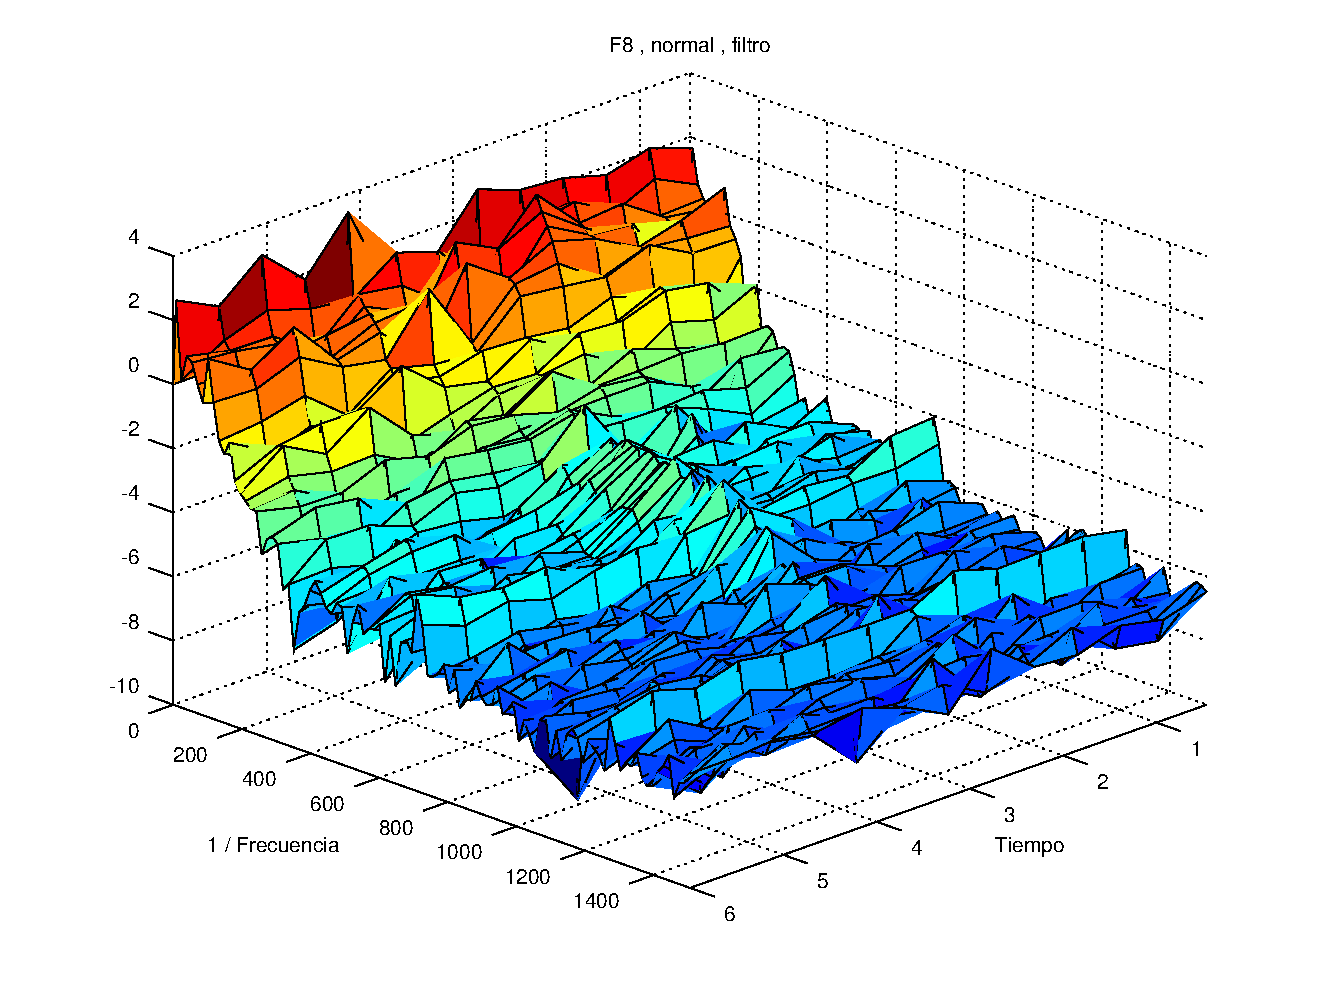
\includegraphics[width=0.5\linewidth]{n8f.pdf} 
&
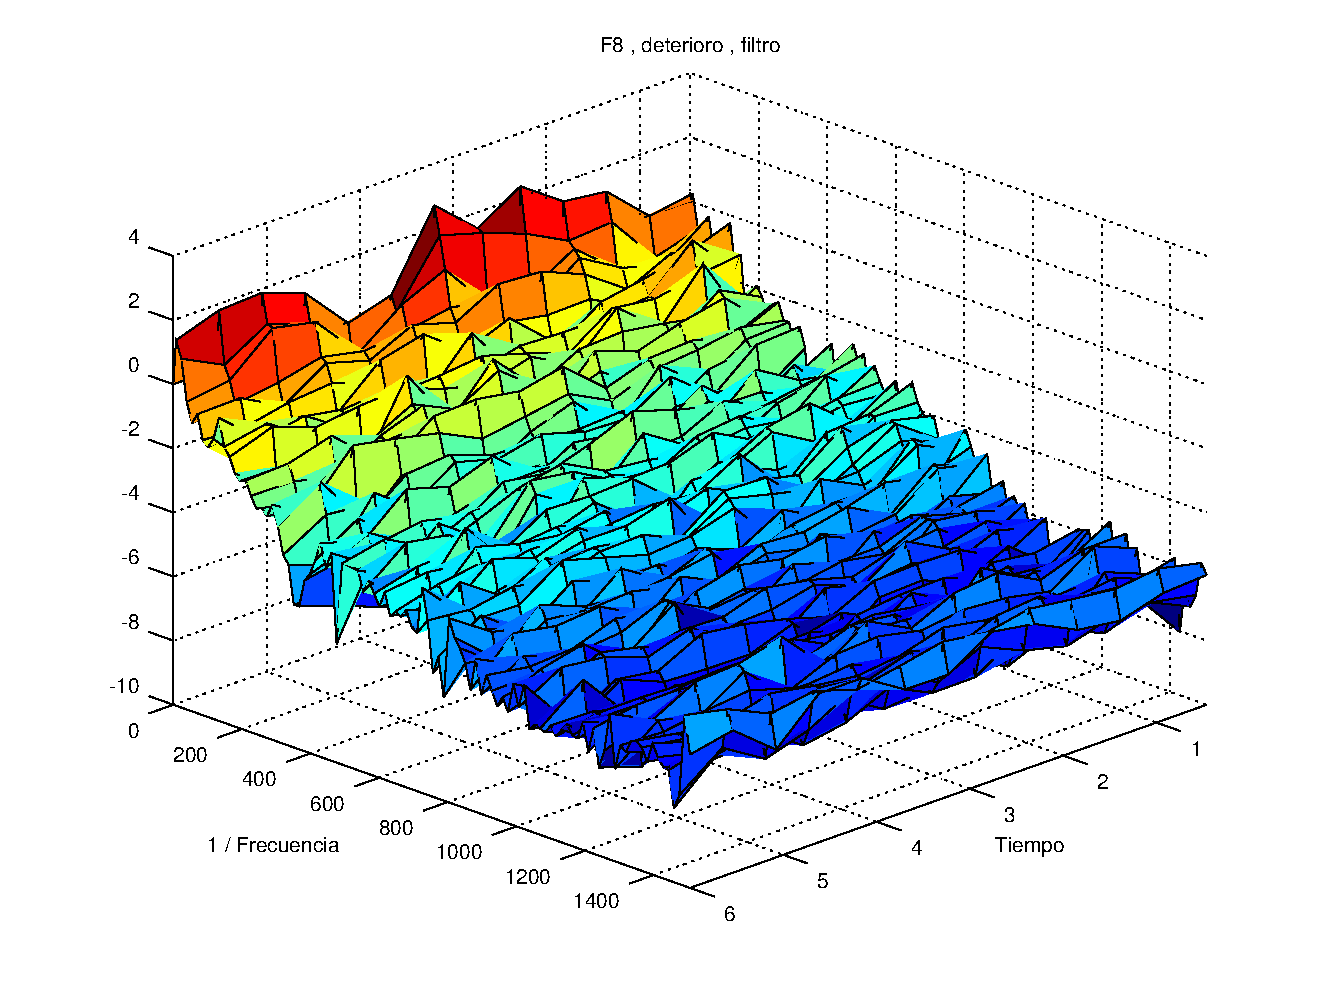
\includegraphics[width=0.5\linewidth]{d8f.pdf} 
\\
\begin{lstlisting}
T      : 0 
I+R    : 5.787895e-09 
T+I+R  : 0 
\end{lstlisting}
&
\begin{lstlisting}
T      : 0.00332259 
I+R    : 0.03502537 
T+I+R  : 0.01598073 
\end{lstlisting}
\end{tabular}

%%%%%%%%%%%%%%%%%%%%%%%%%%%%%%%%%%%%%%%%%%%%%%%%%%%%%%%%%%%%%%%%%%%%%%%%%%%%%%%%%%%%%%%%%%%%%%%%%%%
%%%%%%%%%%%%%%%%%%%%%%%%%%%%%%%%%%%%%%%%%%%%%%%%%%%%%%%%%%%%%%%%%%%%%%%%%%%%%%%%%%%%%%%%%%%%%%%%%%%

\chapter{''Resultados''}

Visually, Rapid Eye Movement (REM) sleep is characterized by REMs, muscle atonia and 
desynchronized EEG activity. When quantitative analyses of the signals are carried out, usually, 
non-linearity and non-stationarity are assumed without an adequate analysis, especially in 
Old Adults (OA). Among the “weak” stationarity tests, the Priestley-Subba Rao (PSR) test 
calculates a “local” spectra that is “valid” only for punctual moments in time. A series of 
“smoothed” frequency filters give information of the time the local spectra is calculated. 
In here, weak REM sleep stationarity by the PSR test was compared to that from Wakefulness (W) 
and Non-REM (NREM) sleep. Methods:  8 Old Adults (OA) 
(age: 67.6 $\pm$ 5.7; education: 8.8 $\pm$ 2.6) 
without depression neither anxiety and with intact daily living activities were selected. Also, 
evaluations with the Mini-Mental State Examination (MMSE, 28.1 $\pm$ 1.8) and a one night 
polysomnography were performed. 30 second epochs were classified according to the AASM and every 
epoch of W, NREM and REM sleep was subjected to PSR tests. Percentages of stationary epochs were 
obtained with respect to the total number of epochs of each stage and Student t-tests were used 
to compare them. Results: The PSR effectively showed different proportions of stationarity 
according to the classification of stages in each subject. In Figure 1, in one OA, epochs with 
stationarity are shown in black and the classification of REM sleep is shown in green. Clearly, 
a lower proportion of stationarity was found in REM sleep vs the other stages. These differences 
reached significance in F7, Fp2, LOG and ROG (p $<$ 0.05, Figure 2). Conclusions: In OA, REM sleep 
showed lower proportions of epochs with stationarity vs. W and NREM sleep at anterior areas, a 
result that could be explained by the tonic and phasic REM sleep. When stationarity measurements 
are planned, it is recommended to differentiate anterior from lateral and posterior areas.

%%%%%%%%%%%%%%%%%%%%%%%%%%%%%%%%%%%%%%%%%%%%%%%%%%%%%%%%%%%%%%%%%%%%%%%%%%%%%%%%%%%%%%%%%%%%%%%%%%%

\section{Resultados del test PSR}

(Por ahora est\'a copiado y pegado un reporte preeliminar sobre los resultados
para tenerlo en cuenta y no olvidarlo; m\'as adelante
escribir\'e una explicaci\'opn adecuada.

Desde el punto de vista formal, se sigue directamente de la descripci\'on del test PSR, y s\'olo
hace falta indicar c\'omo se acomodaron los datos. Desde el punto de vista fisiol\'ogico es m\'as
interesante y extensa la parte que falta.)

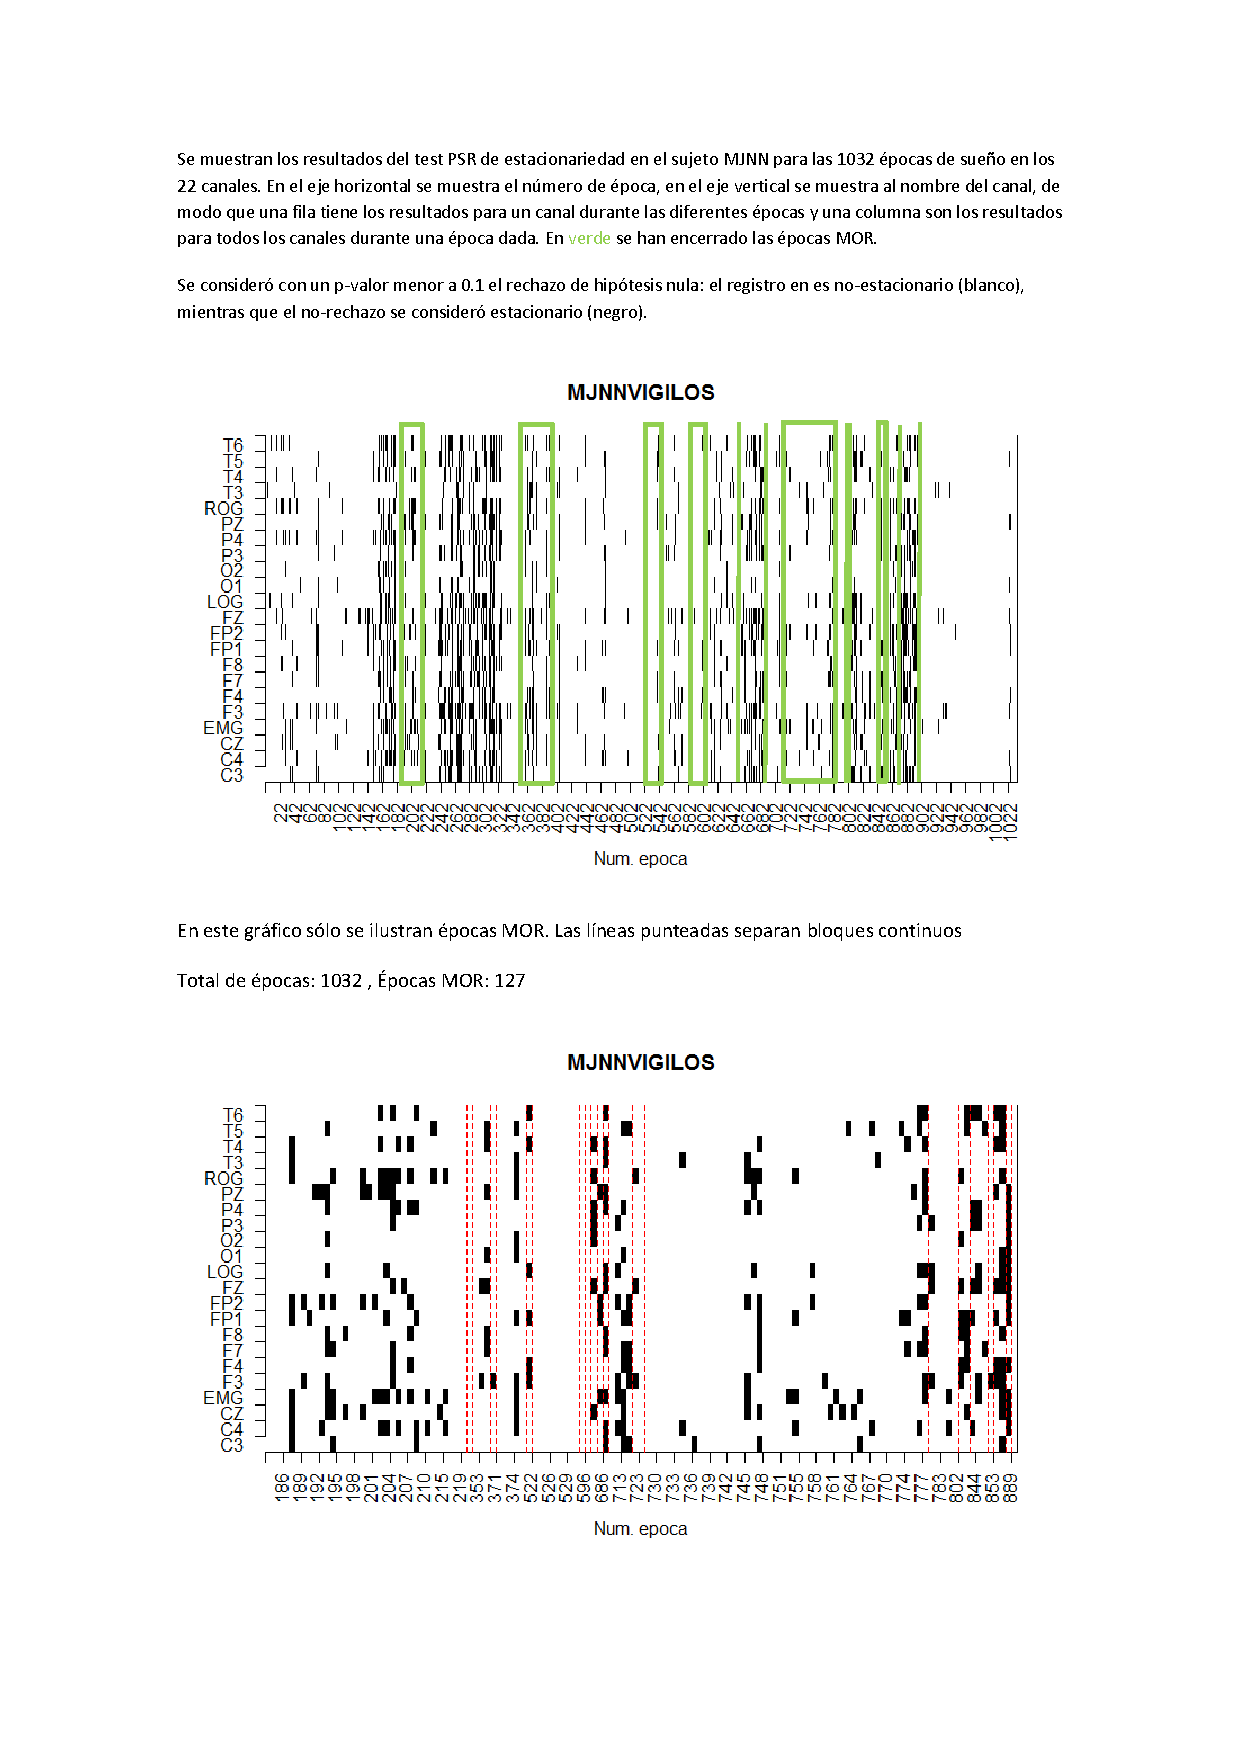
\includepdf[pages={1-},scale=.85]{reporte_de_estacionariedad_170120.pdf}

%%%%%%%%%%%%%%%%%%%%%%%%%%%%%%%%%%%%%%%%%%%%%%%%%%%%%%%%%%%%%%%%%%%%%%%%%%%%%%%%%%%%%%%%%%%%%%%%%%%
%%%%%%%%%%%%%%%%%%%%%%%%%%%%%%%%%%%%%%%%%%%%%%%%%%%%%%%%%%%%%%%%%%%%%%%%%%%%%%%%%%%%%%%%%%%%%%%%%%%

\bibliography{referencias_enciso_alva}{}
%\bibliographystyle{apalike-es}
\bibliographystyle{plain}

%%%%%%%%%%%%%%%%%%%%%%%%%%%%%%%%%%%%%%%%%%%%%%%%%%%%%%%%%%%%%%%%%%%%%%%%%%%%%%%%%%%%%%%%%%%%%%%%%%%
%%%%%%%%%%%%%%%%%%%%%%%%%%%%%%%%%%%%%%%%%%%%%%%%%%%%%%%%%%%%%%%%%%%%%%%%%%%%%%%%%%%%%%%%%%%%%%%%%%%

\end{document}